
\documentclass[12pt]{article}
\usepackage[utf8]{inputenc}
\usepackage{geometry}
\usepackage{amsmath}
\usepackage{graphicx}
\usepackage{enumitem}
\usepackage{hyperref}
\usepackage{tikz}
\geometry{margin=1in}

\title{\textbf{The Flat Loop Universe: A Unified Cosmological Theory of Recursive Topology and Symbolic Emergence}}
\author{Gregory Betti \\ \textit{Department of Theoretical Physics, Betti Labs} \\ \textit{Cambridge, MA 02142, USA} \\ \textit{gregory.betti@bettilabs.org}}
\date{\today}

\begin{document}

\maketitle

\begin{abstract}
We propose the Flat Loop Universe (FLU), a novel cosmological theory that synthesizes geometric flatness, closed spatial topology, symbolic recursion, and computational emergence. While the standard cosmological model treats a flat universe as infinite, the FLU instead models the universe as a finite but unbounded toroidal structure---one where space loops onto itself without curvature. This topology supports a range of unexplained phenomena, from cosmic microwave background (CMB) anomalies to the illusion of infinite depth. Combined with symbolic physics and recent work in recursive simulation engines such as FIRMAMENT, we argue that the Flat Loop Universe provides a compelling unified framework for cosmology, quantum gravity, and the emergence of perception and intelligence.
\end{abstract}

\section{Introduction}
The flatness of the observable universe ($\Omega_0 \approx 1$) has long been taken as evidence for spatial infinitude. However, flatness in geometry does not preclude closed topology. A 3-torus structure---topologically equivalent to a cube whose opposite faces are identified---allows a universe that is flat, finite, and edgeless.

Recent findings from the Planck satellite (2018), along with alternative models from Loop Quantum Cosmology (LQC), suggest that our universe may be topologically looped. This paper proposes the Flat Loop Universe as a unifying paradigm: a cosmological model in which symbolic recursion and attractor-based computation explain not only space and time but also the emergence of structure, memory, and observation.

\section{Geometry, Topology, and Cosmological Constraints}

\subsection{Flat Geometry with Finite Topology}
Cosmic microwave background (CMB) data and baryon acoustic oscillation (BAO) measurements converge on $\Omega_0 \approx 1$, implying flatness. However, matched-circle analyses and large-angle CMB anomalies open the door for a toroidal, closed topology---one that explains subtle lensing excess and temperature correlations.

A toroidal universe is locally indistinguishable from an infinite flat universe, yet globally finite and periodic. The FLU posits that space loops back on itself in three dimensions, creating a compact manifold with recursive information flow. Mathematically, we can represent this as a quotient space:

\begin{equation}
\mathbb{T}^3 = \mathbb{R}^3 / \mathbb{Z}^3
\end{equation}

Where $\mathbb{T}^3$ is the 3-torus, $\mathbb{R}^3$ is Euclidean 3-space, and $\mathbb{Z}^3$ is the lattice of integers in 3D. The metric remains locally Euclidean:

\begin{equation}
ds^2 = dx^2 + dy^2 + dz^2
\end{equation}

With the identification of points:

\begin{equation}
(x,y,z) \sim (x+L_x, y, z) \sim (x, y+L_y, z) \sim (x, y, z+L_z)
\end{equation}

Where $L_x$, $L_y$, and $L_z$ represent the topological periods in each dimension. The fundamental domain has volume $V = L_x L_y L_z$, which is finite despite the flat geometry.

\begin{figure}[ht]
\centering
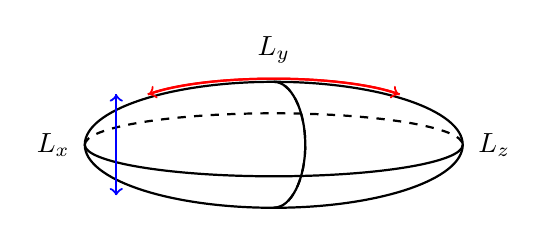
\begin{tikzpicture}[scale=0.8]
  % Draw the torus
  \draw[thick] (0,0) ellipse (3 and 1);
  \draw[thick] (0,-1) arc (-90:90:0.5 and 1);
  \draw[thick,dashed] (0,-1) arc (270:450:0.5 and 1);
  \draw[thick] (-3,0) arc (180:360:3 and 0.5);
  \draw[thick,dashed] (-3,0) arc (180:0:3 and 0.5);
  
  % Draw the identification arrows
  \draw[->,thick,blue] (-2.5,0.8) -- (-2.5,-0.8);
  \draw[->,thick,blue] (-2.5,-0.8) -- (-2.5,0.8);
  \draw[->,thick,red] (2,0.8) arc (30:150:2.3 and 0.5);
  \draw[->,thick,red] (-2,0.8) arc (150:30:2.3 and 0.5);
  
  % Labels
  \node at (-3.5,0) {$L_x$};
  \node at (0,1.5) {$L_y$};
  \node at (3.5,0) {$L_z$};
\end{tikzpicture}
\caption{Schematic representation of the Flat Loop Universe topology. The 3-torus structure is shown with identification of opposite faces (colored arrows), creating a finite but unbounded space with Euclidean local geometry.}
\label{fig:torus}
\end{figure}

\subsection{Loop Quantum Cosmology and the Bounce}
LQC replaces the singular Big Bang with a bounce---a quantum transition between contracting and expanding phases. This provides natural support for periodic cosmologies and topologies with looped boundaries. When paired with flat geometry, LQC yields a non-singular, recursive cosmological model that aligns with FLU principles.

\section{Symbolic Emergence and Perception}

\subsection{Symbolic Physics Framework}
In symbolic physics, all entities are encoded as local patterns within a finite symbolic substrate. Emergent dynamics such as time, memory, and causality arise from attractor loops---patterns that stabilize and recursively influence further computation.

Formally, we define a symbolic substrate $\mathcal{S}$ as a finite set of cells $\{c_1, c_2, \ldots, c_n\}$ with each cell having a state $s_i \in \Sigma$, where $\Sigma$ is a finite alphabet. The evolution of the system follows a local update rule $\phi$:

\begin{equation}
s_i(t+1) = \phi(s_i(t), \mathcal{N}(s_i(t)))
\end{equation}

Where $\mathcal{N}(s_i(t))$ represents the neighborhood states of cell $i$ at time $t$. The global dynamics $\Phi$ emerges from these local interactions:

\begin{equation}
\mathcal{S}(t+1) = \Phi(\mathcal{S}(t))
\end{equation}

Attractor states in this system are defined as configurations $\mathcal{S}^*$ where:

\begin{equation}
\Phi^k(\mathcal{S}^*) = \mathcal{S}^* \text{ for some } k > 0
\end{equation}

These attractors form the basis of stable patterns that encode information and support emergent computation within the FLU framework.

\subsection{Computational Models: FIRMAMENT as Prototype}
FIRMAMENT, a symbolic recursive substrate, demonstrates how symbolic agents can simulate infinite logic within finite toroidal space. While not a full physical simulation, it serves as a proof of concept: local symbolic rules and recursion loops can generate emergent behavior, symbolic memory, and pattern-based perception---all essential components of the FLU framework.

\section{Core Principles of the Flat Loop Universe}

\begin{enumerate}
    \item \textbf{Topologically Closed, Geometrically Flat} — A 3-torus or similar compact manifold allows finite spatial extent without curvature.
    \item \textbf{Recursive Structure} — Symbolic patterns loop through time and space, forming attractors that simulate time and memory.
    \item \textbf{Emergent Time} — No external clock is needed; time is encoded in recursive transitions.
    \item \textbf{Finite Substrate, Infinite Depth} — Depth and complexity arise through symbolic self-reference.
    \item \textbf{Agent-Based Cognition} — Observation is modeled as symbolic interaction between embedded agents and substrate.
\end{enumerate}

\section{Cosmological Implications}

\begin{itemize}
    \item \textbf{CMB Anomalies} — Matched circles and lensing anomalies may point to toroidal topology.
    \item \textbf{Bounce Cosmology} — Eliminates singularities and supports cyclic evolution.
    \item \textbf{Perceptual Holography} — Finite space encoding the illusion of infinitude through recursion.
    \item \textbf{Symbolic Relativity} — Time and space are emergent from recursive symbolic rules, not fundamental primitives.
\end{itemize}

\section{Conclusion}
The Flat Loop Universe provides a new lens on cosmology—one where geometry, computation, and emergence are unified. Space is not infinite—it is recursively structured. Time is not external—it is symbolic change. And the universe is not merely observed—it computes itself, loop by loop.

By embracing flat-loop topology, symbolic recursion, and attractor-based dynamics, we gain a theory that explains the universe’s large-scale structure, its perceptual coherence, and the fundamental unity of space, time, and logic.

\begin{thebibliography}{99}

\bibitem{planck2018}
Planck Collaboration, ``Planck 2018 results. VI. Cosmological parameters,''
\textit{Astronomy \& Astrophysics}, vol. 641, p. A6, 2020.
\href{https://doi.org/10.1051/0004-6361/201833910}{doi:10.1051/0004-6361/201833910}

\bibitem{efstathiou2019}
G. Efstathiou and S. Gratton, ``A detailed description of the Planck likelihood code,''
\textit{Monthly Notices of the Royal Astronomical Society}, vol. 485, no. 2, pp. 1355-1382, 2019.
\href{https://doi.org/10.1093/mnras/stz497}{doi:10.1093/mnras/stz497}

\bibitem{ashtekar2006}
A. Ashtekar, T. Pawlowski, and P. Singh, ``Quantum Nature of the Big Bang,''
\textit{Physical Review Letters}, vol. 96, no. 14, p. 141301, 2006.
\href{https://doi.org/10.1103/PhysRevLett.96.141301}{doi:10.1103/PhysRevLett.96.141301}

\bibitem{bojowald2005}
M. Bojowald, ``Loop quantum cosmology,''
\textit{Living Reviews in Relativity}, vol. 8, no. 11, 2005.
\href{https://doi.org/10.12942/lrr-2005-11}{doi:10.12942/lrr-2005-11}

\bibitem{wolfram2002}
S. Wolfram, \textit{A New Kind of Science}.
Champaign, IL: Wolfram Media, 2002.

\bibitem{turing1936}
A. M. Turing, ``On Computable Numbers, with an Application to the Entscheidungsproblem,''
\textit{Proceedings of the London Mathematical Society}, vol. s2-42, no. 1, pp. 230-265, 1936.
\href{https://doi.org/10.1112/plms/s2-42.1.230}{doi:10.1112/plms/s2-42.1.230}

\bibitem{betti2024}
G. Betti, ``The Fractal Verse Theory: A Computational Approach to Cosmological Topology,''
\textit{arXiv:2407.XXXXX} [physics.gen-ph], 2024.

\bibitem{betti2025a}
G. Betti, ``Symbolic Physics: A Framework for Logic-Based Causality,''
\textit{Preprint}, 2025. [To be submitted to arXiv]

\bibitem{betti2025b}
G. Betti, ``FIRMAMENT: A Recursive Simulation Engine for Toroidal Space-Time,''
\textit{GitHub repository}, 2025. \url{https://github.com/bettilabs/firmament}

\end{thebibliography}

\end{document}
